\documentclass[11pt, titlepage]{article}
\usepackage{amsmath,amsthm,amssymb}
\usepackage{hyperref, pgf, tikz}
\usepackage{fancyhdr}
\usetikzlibrary{arrows}
\usepackage[margin=1.25in]{geometry}
\usepackage{graphicx}                     
\pagestyle{fancy}
\usepackage{array}
%\usepackage{wrapfig}

\lhead{Lab \#1}
\rhead{\thepage}
\cfoot{}

\title{\Huge{Newton's Second Law: The Atwood Machine} \\ \ \\ \huge Lab \#1}
\author{\Large{Alon Levin} \\ \emph{Lab Partner: Avery Karlin}}
\date{\today}
\begin{document}

\maketitle

\begin{center}
\LARGE Newton's Second Law: The Atwood Machine
\end{center}

\section*{Objective}
The objective of this lab is to experimentally obtain the aceleration of a system of masses on an Atwood machine, and to describe how it changes in response to (1) mass variations with a constant unbalanced force and (2) foce variations with constant mass.

\section*{Introduction}
\subsection*{Atwood Machine}
The Atwood machine was named after George Atwood (1746-1807), its designer. The machine consists of two masses hanging on a string about a pulley or a pulley system, and was used to experimentally determine acceleration due to gravity on Earth ($g = 9.81 \frac{m}{s^2}$) by measuring the relatively slow uniform acceleration of the system.

\subsection*{Newton's Second Law}
Newton's Second Law states that the acceleration $a$ of a system is directly proportional to the net force \textbf{$F_{net}$} acting on the system, and inversely proportional to the total mass $m$ of the system. In other words, $$ a \propto \frac{F_{net}}{m}$$
Rewritten, the formula gains its more common form: $$F_{net} = ma$$

On an Atwood machine, the force of gravity ($F_g = mg$) works in opposite directions, as the force of the masses pulling on each respective side of the pulley causes tension to pull on both masses. Since the masses are connected and indirectly acting on each other, the total acceleration for the system is constant. However, as this is not a perfect system and is subjected to real world constraints, we must subtract the force of friction (both from the pulley, acting on the string, and from the surrounding air, acting on the entire system) and add the mass of the pulley to the total mass in order to gain accurate results.

Based on these facts, we attain the following: $$F_{net} = (m_1 + m_2 + m_{pulley})a = m_1g - m_2g - f$$where $f$ is the force of friction. This can then be rewritten as $$a = \frac{(m_2 - m_1)g - f}{m_1 + m_2 + m_{pulley}}.$$ 

In order to find the value of the frictional force, we must find a solution for when acceleration is equal to 0. If the frictional force $f$ of the system is divided by the gravitational constant $g$ to find the mass $m_f$ that must be subtracted out due to friction, we can rewrite the previous equation as: $$a = \frac{(m_2 - m_1 - m_f)g}{m_1 + m_2 + m_{pulley}}$$

The acceleration (assuming that it is constant) of the actual experimental system is found by determining the time it takes one of the masses to fall a specific distance and using the standard distance equation $y = v_0t + \frac{1}{2}at^2$ In the case that the mass starts from rest, the equation could be rewritten in order to solve for acceleration in the following way: $$a = \frac{2y}{t^2}.$$

\section*{Procedure}
After constructing the Atwood machine (see Figure 1), two equal masses should be attached to each side. Note that if a light force is temporarily applied to one side, the system will begin to accelerate. To counteract this, additional mass should be added to one side (designated the \emph{descending side}) until a slight downard tug on it will result in motion at constant velocity, signifying that the system's acceleration $a=0$; this added mass is $m_f$, the mass needed to compensate for friction. Now, we add mass to the descending side and time how long it takes for this mass to fall a specific distance. We repeat this with several different masses on both sides, preserving the relative mass but requiring different frictional masses, and record the resultant acceleration for each trial.

For the next portion, the experiment is reset with equal masses put on both sides again. Once the frictional mass is determined, a certain amount of mass is moved from one side to the other, thus creating an unbalanced force while keeping the total mass constant. Each additional trial has a greater imbalance of mass than the previous. Once again, the masses are released, and the time required for one to travel a certain distance is used to measure the resultant acceleration.

\pagebreak
\begin{figure}[!ht]
\centering
\vspace*{1.5cm}
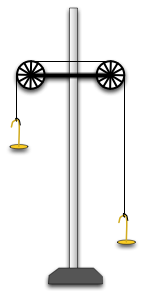
\includegraphics[scale=1.5, angle=0]{lab01.jpg}
\caption{Setup used for this experiment}
\end{figure}

\pagebreak
\section*{Data}
Mass of the pulley, measured:$$m_{pulley} = 31.6 g$$
\begin{center}
\begin{tabular}
{|m{7em}|m{7em}|m{7em}|m{7em}|m{7em}|}
\hline
Trial & 1 & 2 & 3 & 4 \\
\hline
Descending Mass, $m_2$ (kg) & 0.06636 & 0.165 & 0.26636 & 0.3673\\
\hline
Ascending Mass, $m_1$ (kg) & 0.055 & 0.150 & 0.250 & 0.350\\
\hline
Distance of Travel, $y$ (m) & 0.8984 & 0.855 & 0.605 & 0.61\\
\hline
Time of Travel, Run 1, $t_1$ (s) & 1.47 & 2.1 & 2.54 & 3.28\\
\hline
Time of Travel, Run 2, $t_2$ (s) & 1.21 & 2.27 & 2.48 & 3.4\\
\hline
Time of Travel, Run 3, $t_3$ (s) & 1.31 & 2.18 & 2.44 & 3.55\\
\hline
Average Time, $t_{avg}$ (s) & 1.33 & 2.183 & 2.486 & 3.41\\
\hline
Measured Acceleration, $a_m$ ($kgm/s^2$) & 1.015 & 0.359 & 0.196 & 0.105\\
\hline
Total Mass, $m_t$ (kg) & 0.1529 & 0.3466 & 0.547 & 0.7489\\
\hline
Frictional Mass, $m_f$ (kg) & 0.00136 & 0.005 & 0.00636 & 0.0073\\
\hline
Net Force, $F_{net}$ (N) & 0.098 & 0.163 & 0.149 & 0.098\\ 
\hline
Theoretical Acceleration, $a_t$ ($kg*m/s^2$) & 0.64 & 0.47 & 0.27 & 0.131\\
\hline
Percent Acceleration Error (\%) & 58.59 & 23.62 & 27.4 & 19.7\\
\hline
\end{tabular}
\begin{figure}[!ht]
\caption{\emph{Varying the Total Mass}}
\end{figure}
\end{center}
\pagebreak
\section*{Data (cont.)}
\begin{center}
\begin{tabular}
{|m{7em}|m{7em}|m{7em}|m{7em}|m{7em}|}
\hline
Trial & 5 & 6 & 7 & 8 \\
\hline
Descending Mass, $m_2$ (kg) & 0.2673 & 0.2693 & 0.2713& 0.2763\\
\hline
Ascending Mass, $m_1$ (kg) & 0.259 & 0.257 & 0.255 & 0.25\\
\hline
Distance of Travel, $y$ (m) & 0.61 & 0.61 & 0.61 & 0.61\\
\hline
Time of Travel, Run 1, $t_1$ (s) & 9.16& 4.58& 2.75& 2.1\\
\hline
Time of Travel, Run 2, $t_2$ (s) & 6.35& 3.6 & 3.16 & 2\\
\hline
Time of Travel, Run 3, $t_3$ (s) & 8.15& 4.21 & 3.03 & 2.13\\
\hline
Average Time, $t_{avg}$ (s) & 7.88 & 4.13 & 2.98 & 2.076 \\
\hline
Measured Acceleration, $a_m$ ($m/s^2$) & 0.0196 & 0.0715 & 0.137& 0.283\\
\hline
Total Mass, $m_t$ (kg) & 0.5589 & 0.5589 & 0.5589 & 0.5589\\
\hline
Frictional Mass, $m_f$ (kg) & 0.0073 & 0.0073 & 0.0073 & 0.0073\\
\hline
Net Force, $F_{net}$ (N) & 0.0098 & 0.049 & 0.0882 & 0.1862\\ 
\hline
Theoretical Acceleration, $a_t$ ($m/s^2$) & 0.0175 & 0.0877 & 0.158 & 0.333 \\
\hline
Percent Acceleration Error (\%) & 12 & 18.5 & 13.3 & 15.01 \\
\hline
\end{tabular}
\begin{figure}[!ht]
\caption{\emph{Varying the Unbalanced Force}}
\end{figure}
\end{center}

\pagebreak
\section*{Discussion}
\subsection*{Sample Calculations}
$$t_{avg} = \frac{t_1 + t_2 + t_3}{3} = \frac{1.47 + 1.21 + 1.31}{3} = 1.33$$
$$a = \frac{2y}{t^2} = \frac{2*0.8984}{1.33^2} = 1.015$$
$$m_t = m_1 + m_2 + m_{pulley} = 0.06636 + 0.055 + 0.0316 = 0.1529$$
$$F_{net} = (m_2 - m_1 - m_f)g = (0.06636 - 0.055 - 0.00136)(9.8) = 0.098$$
$$a_t = \frac{F_{net}}{m_t} = \frac{0.098}{0.1529} = 0.64$$
$$\text{Percent Acceleration Error} = \frac{|a_t - a_m|}{a_t}*100\% = \frac{|0.64 - 1.015|}{0.64}*100\% = \frac{0.375}{0.64}*100\% = 58.59\%$$

\subsection*{Non-Measured Data}
\begin{center}
\begin{tabular}
{|m{7em}|m{7em}|m{7em}|m{7em}|m{7em}|}
\hline
Trial & 1 & 2 & 3 & 4 \\
\hline
Average Time, $t_{avg}$ (s) & 1.33 & 2.183 & 2.486 & 3.41\\
\hline
Measured Acceleration, $a_m$ ($kgm/s^2$) & 1.015 & 0.359 & 0.196 & 0.105\\
\hline
Total Mass, $m_t$ (kg) & 0.1529 & 0.3466 & 0.547 & 0.7489\\
\hline
Net Force, $F_{net}$ (N) & 0.098 & 0.163 & 0.149 & 0.098\\ 
\hline
Theoretical Acceleration, $a_t$ ($kg*m/s^2$) & 0.64 & 0.47 & 0.27 & 0.131\\
\hline
\textbf{Percent Acceleration Error (\%)} & 58.59 & 23.62 & 27.4 & 19.7\\
\hline
\end{tabular}
\begin{figure}[!ht]
\caption{Non-Measured Data for \emph{Varying the Total Mass}}
\end{figure}
\end{center}
\subsection*{Non-Measured Data (cont.)}
\begin{center}
\begin{tabular}
{|m{7em}|m{7em}|m{7em}|m{7em}|m{7em}|}
\hline
Trial & 5 & 6 & 7 & 8 \\
\hline
Average Time, $t_{avg}$ (s) & 7.88 & 4.13 & 2.98 & 2.076 \\
\hline
Measured Acceleration, $a_m$ ($m/s^2$) & 0.0196 & 0.0715 & 0.137& 0.283\\
\hline
Total Mass, $m_t$ (kg) & 0.5589 & 0.5589 & 0.5589 & 0.5589\\
\hline
Net Force, $F_{net}$ (N) & 0.0098 & 0.049 & 0.0882 & 0.1862\\ 
\hline
Theoretical Acceleration, $a_t$ ($m/s^2$) & 0.0175 & 0.0877 & 0.158 & 0.333 \\
\hline
\textbf{Percent Acceleration Error (\%)} & 12 & 18.5 & 13.3 & 15.01 \\
\hline
\end{tabular}
\begin{figure}[!ht]
\caption{Non-Measured Data for \emph{Varying the Unbalanced Force}}
\end{figure}
\end{center}

\subsection*{Analysis}
For the first portion of the lab, there seems to be an inverse relationship between average time of descent and percent acceleration error. Considering that as the total mass increased, the time for descent increased, it could be an issue of improper timing; the rapidity with which the masses of the earlier trials fell could have led to greater inaccuracy in measurement.

As well, the qualities of the pulleys should be taken into account. The frictional force was estimated by manually finding the frictional mass using nonstandard weights, creating room for error; likewise, drag could have had a slowing effect on the measured acceleration, which is consistent with all but the $1^{st}$ and $5^{th}$ trials. We also should not underestimate mechanical failures of the pulley itself, as it could have been the case that the system could have slipped or caught onto something at any point during the experiment.

The final possible source of error is from the equations themselves; the equations used in calculations were intended for a point mass rather than the physical masses that we actually used. This error would affect the higher-massed trials more than the ones with lower mass, as the higher the mass and volume of the weight, the less it acts as as a point and the more it affects the data.

\section*{Conclusion}
As the mass on each side of the pulley (before frictional mass was added) increased from 0.05 kg to 0.35 kg in 0.1 kg increments, the acceleration of the system went from 1.015 $m/s^2$ (58.59\% error), to 0.359 $m/s^2$ (23.62\% error), to 0.196 $m/s^2$ (27.4\% error), to 0.105 $m/s^2$ (19.7\% error).

As the difference in mass increased from 0.002 kg, to 0.006 kg, to 0.01 kg, to 0.02 kg, the acceleration of the system went from 0.0196 $m/s^2$ (12\% error), to 0.0715 $m/s^2$ (18.5\% error), to 0.137 $m/s^2$ (13.3\% error), to 0.283 $m/s^2$ (15.01\% error). 

\end{document}